\section{Introduction}

% \IEEEPARstart{R}{eal-time} object detection has long been at the forefront of computer vision research~\cite{realtime_survey,yolo_survey}, aiming to localize and classify objects within images with minimal latency, which is critical for a wide range of applications, \eg, industrial inspection, autonomous driving, and video surveillance~\cite{yolo_survey_1_8}. In recent years, single‑stage CNN detectors, which integrate region proposal, classification, and regression into a unified end‑to‑end network, have come to dominate the field \cite{survey_20}. Among these, the You Only Look Once (YOLO) series \cite{yolov1,yolov2,yolov3,yolov4,yolov5,yolov6,yolov7,yolov8,yolov9,yolov10,yolo11,yolov12} has become the mainstream framework due to its excellent balance achieved between inference speed and detection accuracy.
\IEEEPARstart{R}{eal-time} object detection has long been at the forefront of computer vision research~\cite{obj_det_survey,survey_20y}, aiming to localize and classify objects within images with minimal latency, which is critical for a wide range of applications, \eg, industrial anomaly detection, autonomous driving, and video surveillance~\cite{yolo_based_survey}. Recent years have witnessed the dominance of single‑stage CNN detectors that integrate region proposal, classification, and regression into a unified end‑to‑end framework in this field~\cite{rcnn,maskrcnn,yolov1,rt_detr}. Among them, YOLO (You Only Look Once) series~\cite{yolov1,yolov2,yolov3,yolov4,yolov5,yolov6,yolov7,yolov8,yolov9,yolov10,yolo11,yolov12} has become mainstream due to its excellent balance between inference speed and accuracy.

% wever, to date, YOLO models, from the pure convolutional architecture of YOLO11 and earlier versions to the area‑based self‑attention \cite{yolov12} introduced in YOLOv12, have failed to adequately capture the high‑order, many‑to‑many visual semantic associations that are widely present in the scenes. High‑order visual associations refer to complex group structures formed by interactions between three or more objects or regions within the same spatio-temporal context, such as simultaneous interactions among multiple objects or multifaceted semantic couplings between objects and their backgrounds. Pure convolutional operations inherently perform local aggregation within a fixed receptive field, constrained by kernel size and network depth. Although area‑based self‑attention extends the receptive field, it must resort to localized windows as a compromise due to its heavy computational cost, and thus cannot achieve full global perception. Furthermore, the computing process of self‑attention can be viewed as pairwise interactions on a fully connected semantic graph, limiting it to modeling binary relationships and preventing it from simultaneously representing and aggregating many‑to‑many interactions within a single mechanism. Consequently, existing YOLO architectures often encounter performance bottlenecks in complex scenarios, making further improvements in detection accuracy and robustness difficult.
\begin{figure}[!tbp]
    \centering
    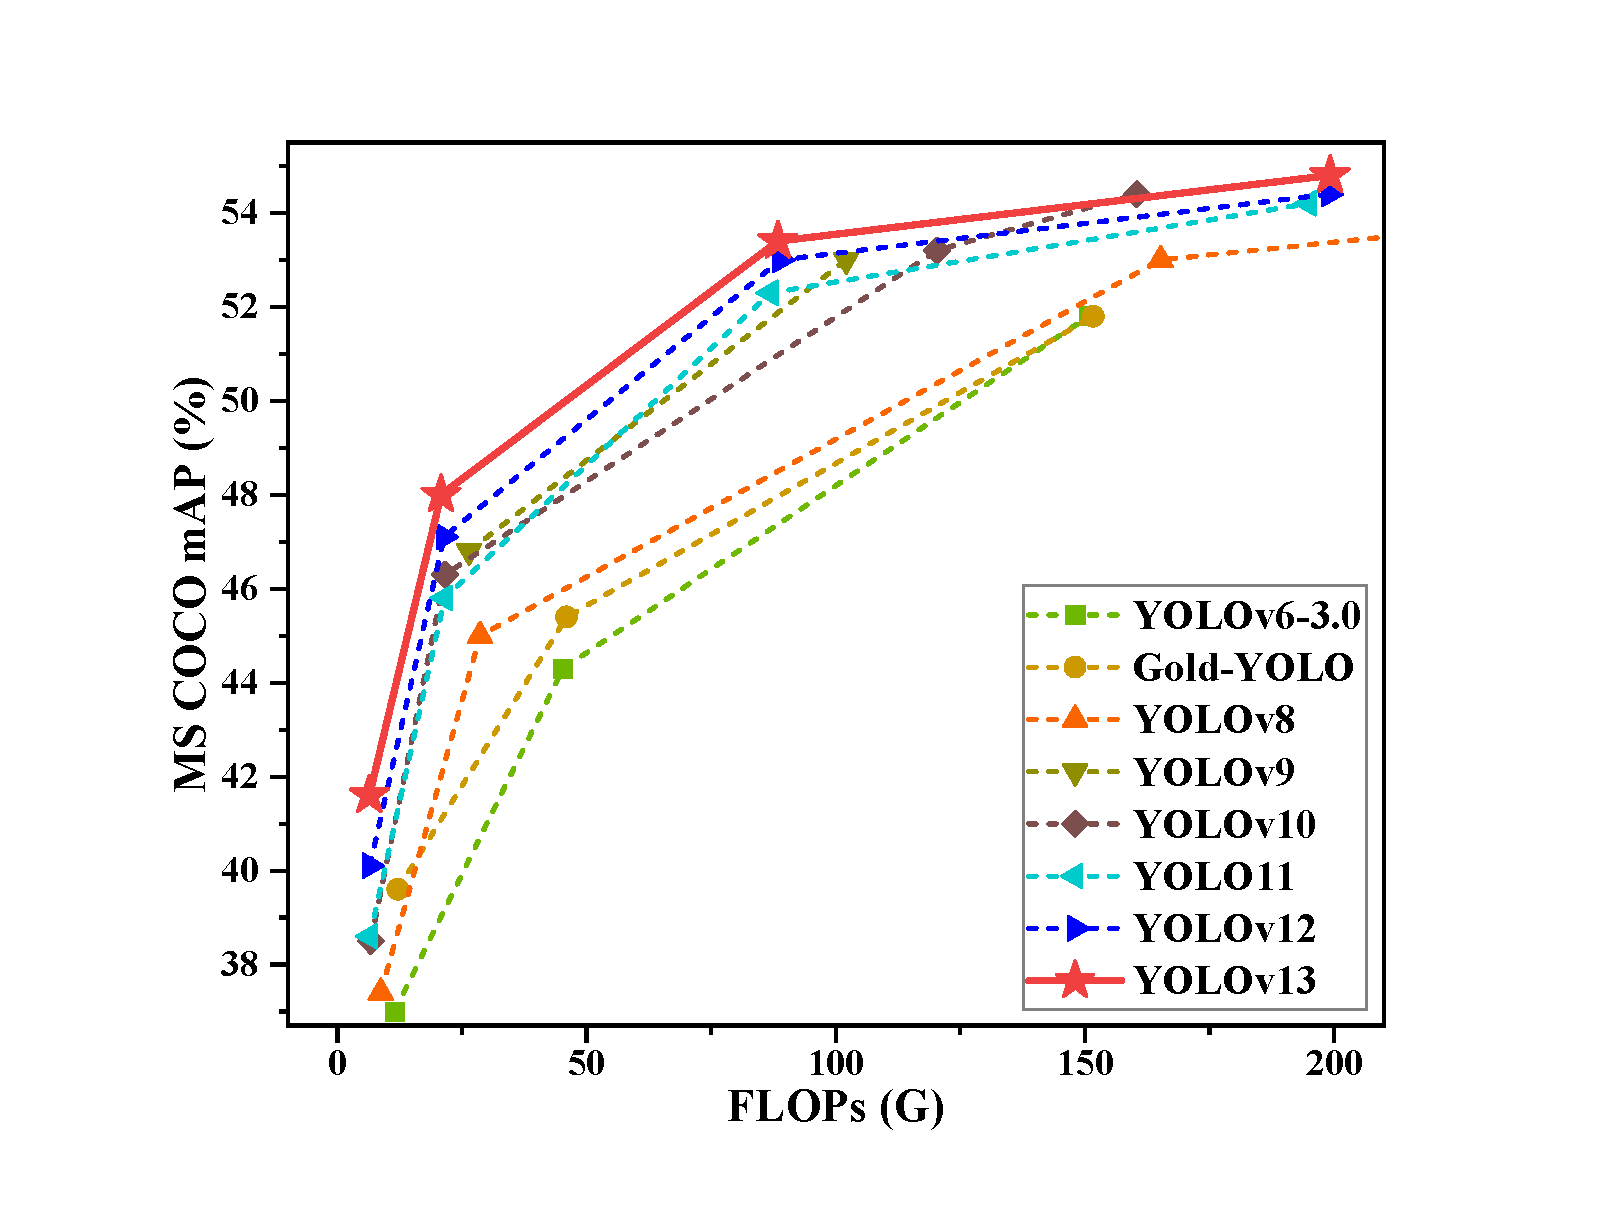
\includegraphics[width=1\linewidth]{figures/fig1.pdf}
    \vspace{-0.6cm}
    \caption{Comparison of our proposed YOLOv13 model with previous YOLO models on the MS COCO dataset. Our proposed model can achieve higher detection accuracy with lower computational complexity.}
     \vspace{-0.6cm}
    \label{fig:fig1}
\end{figure}
From the early YOLO versions to the recent YOLO11 model, architectures centered on convolution have been adopted, aiming to extract image features and achieve object detection through differently designed convolutional layers. The latest YOLOv12 model~\cite{yolov12} further leverages an area-based self-attention mechanism to enhance the representation capability of the model. On the one hand, convolutional operations inherently perform local information aggregation within a fixed receptive field. Thus, the modeling capacity is constrained by the kernel size and network depth. On the other hand, although the self-attention mechanism extends the receptive field, its high computational cost necessitates the use of local area-based computation as a trade-off, thereby preventing adequate global perception and modeling. In addition, the self-attention mechanism can be regarded as the modeling of pairwise pixel correlations on a fully-connected semantic graph, which inherently limits its capacity to capturing only binary correlations and prevents it from representing and aggregating multi-to-multi high-order correlations. Therefore, the architecture of existing YOLO models restricts their capability to model global high-order semantic correlations, leading to performance bottlenecks in complex scenarios. Hypergraphs can model multi-to-multi high-order correlations. Different from traditional graphs, each hyperedge in a hypergraph connects multiple vertices, thus enabling the modeling of correlations between multiple vertices. Some studies~\cite{vihgnn,hgvit,hgformer} have demonstrated the necessity and validity of using hypergraph to model multi-pixel high-order correlations for visual tasks including object detection. However, existing methods simply use manually set threshold parameter values to determine whether pixels are correlated based on pixel feature distances, \ie, pixels with feature distances below a specific threshold are deemed to be correlated. This manual modeling paradigm makes it difficult to cope with complex scenes and leads to additional redundant modeling, resulting in limited detection accuracy and robustness.

To address the above-mentioned challenges, we propose \textbf{YOLOv13}, a novel, real-time, breakthrough end-to-end object detector. Our proposed YOLOv13 model extends traditional region-based pairwise interaction modeling to global high-order correlation modeling, enabling the network to perceive deep semantic correlations across spatial positions and scales, which significantly enhances detection performance in complex scenarios. Specifically, to overcome the limitations in robustness and generalization caused by the handcrafted hyperedge construction in existing methods, we propose a novel \textbf{Hyper}graph-based \textbf{A}daptive \textbf{C}orrelation \textbf{E}nhancement mechanism, named \textbf{HyperACE}. HyperACE takes pixels in multi-scale feature maps as vertices and adopts a learnable hyperedge construction module to adaptively explore high-order correlations between vertices. Then, a message-passing module with linear complexity is leveraged to effectively aggregate multi-scale features with the guidance of high-order correlations to achieve effective visual perception of complex scenarios. In addition, low-order correlation modeling is also integrated in HyperACE for complete visual perception. Building on HyperACE, we propose a novel YOLO architecture containing a \textbf{Full}‑\textbf{P}ipeline \textbf{A}ggregation‑and-\textbf{D}istribution paradigm, named \textbf{FullPAD}. Our proposed FullPAD aggregates multi-level features extracted from the backbone network using the HyperACE mechanism, and then distributes the correlation-enhanced features to the backbone, neck, and detection head to achieve fine‑grained information flow and representational synergy across the entire pipeline, which significantly improves the gradient propagation and enhances the detection performance. Finally, to reduce model size and computational cost without sacrificing performance, we propose a series of lightweight feature extraction blocks based on depthwise separable convolutions. By replacing large‑kernel vanilla convolutional blocks with the depthwise separable convolution blocks, faster inference speed and reduced model size can be achieved, resulting in a better trade-off between efficiency and performance. To validate the effectiveness and efficiency of our proposed model, we conduct extensive experiments on the widely used MS COCO benchmark~\cite{mscoco}. The quantitative and qualitative experimental results demonstrate that our proposed method outperforms all previous YOLO models and variants while remaining lightweight. In particular, YOLOv13‑N/S achieve 1.5\%/0.9\% and 3.0\%/2.2\% mAP improvements compared to YOLOv12‑N/S and YOLO11‑N/S, respectively. Ablation experiments further demonstrate the effectiveness of each proposed module.

% To address these limitations, we propose YOLOv13, which leverages efficient high‑order visual association modeling to enable the network to perceive deep semantic relationships across positions and scales. First, we design the Soft Hypergraph‑based Visual Association Capturing (HyperVAC) module. This module treats the pixel-level features in multi‑scale feature maps as hypergraph nodes, employs learnable soft hyperedges to dynamically construct high‑order associations between nodes, and uses a linear‑complexity message passing mechanism to efficiently aggregate many‑to‑many interactions, thereby fully exploiting the feature maps’ inherent complex interdependencies. Building on this, we redesign the YOLO architecture and introduce the Full‑Pipeline Aggregation‑Distribution (FullPAD) mechanism: centered on HyperVAC, it uniformly aggregates multi‑level backbone features within the hypergraph space and then redistributes the enhanced high‑order association features throughout the Backbone, Neck, and Detection Head, achieving fine‑grained information flow and representational synergy across the entire pipeline. This significantly improves the gradient propagation and enhances the detection performance. Finally, to reduce model size and inference cost without sacrificing any accuracy, we replace all large‑kernel convolutional blocks (non‑$1\times 1$ convolutions) with more efficient depthwise separable convolutional blocks (DS‑C3k). On the MSCOCO benchmark, our approach outperforms all previous YOLO variants while remaining lightweight. In particular, YOLOv13‑S achieves a XX\% and XX\% mAP improvement over YOLO11‑S and YOLOv12‑S, respectively.

Our contributions are summarized as follows:
\begin{itemize}
    \item We propose YOLOv13, a superior real-time end-to-end object detector. Our YOLOv13 model uses adaptive hypergraphs to explore potential high-order correlations, and achieves accurate and robust detection based on effective information aggregation and distribution with the guidance of high-order correlations.
% Our YOLOv13 model is based on hypergraph-based global correlation enhancement mechanism and full-pipeline aggregation‑and-distribution paradigm to effectively aggregate, enhance, and distribute multi-scale features with the guidance of adaptive higher-order correlations.
    \item We propose HyperACE mechanism to capture the latent high-order correlations in complex scenes based on adaptive hypergraph computation and achieve feature enhancement based on correlation guidance. We propose a FullPAD paradigm to enable multi‑scale feature aggregation and distribution within the entire pipeline, enhancing information flow and representational synergy. We propose a series of lightweight blocks based on depthwise separable convolutions to replace large-kernel vanilla convolutional blocks, significantly reducing the number of parameters and computational complexity.
    \item We conduct extensive experiments on the MS COCO benchmark. The experimental results demonstrate that our YOLOv13 achieves state-of-the-art detection performance while maintaining lightweight.
\end{itemize}


